\clearpage
\section{Theory}

\subsection{Dislocation lines}

Several investigations have documented that dislocations in silicon give rise to characteristic photoluminescence (PL) spectra below the band edge. First showed in \cite{drozdov76} which labeled them D1 (0.812eV), D2 (0.875eV), D3 (0.934eV) and D4 (1.000eV). The samples where deformed at 850$^\circ$ C by bending, so that dislocation densities was inhomogeneous along the samples. \cite{drozdov76} states that the intensity of theese lines increase when the dislocation-rich parts of the crystal is approached. At the same time the intensity of the intrinsic characteristics decrease. The distance between D1-D4 (62 $\pm$ 3 meV) corresponds to the energy of the optical phonons in silicon \cite{drozdov76}. \cite{drozdov76} reports D1 and D2 are dominant in heavily deformed Si crystals, while D3 and D4 predominate in weakly deformed Si. A similar result was also reported by \cite{lee09} for small angle grain boundaries using cathodoluminescence.

\cite{sauer85} suggest that D1-D4 are due to dislocations which have been frozen in under low-shear stress. Photoluminescence under uniaxial stress shows that D1/D2 originate in the tetragonal defect with random orientation relative to <100> directions. \cite{sauer85} conclude that D3 and D4 are closely related, whereas the independent D1/D2 centers might be deformation-produced point defects in the strain region of dislocations. New lines D5 and D6 emerge when high-temperature, low-stress deformation is followed by low-temperature, high-stress deformation. \cite{sauer85} propose that line D5 is due to straight dislocations and D6 is due to stacking faults. \cite{sauer85} also suggest that D3/D4 photoluminescence is much more characteristic of the dislocations themselves than the D1/D2 emission lines. \cite{weronek91} state that D5 is correlated with electron-hole recombination at localized centers on separate partial dislocations. After annealing at moderate temperatures (T > 360$^\circ$C) the new lines merge into D4 \cite{weronek91}.


The origin of D1 and D2 is not clear. It has been argued that they originate in electronic transition at the geometrical kinks on dislocations \cite{suezawa83}, point defects \cite{sauer85} and impurities \cite{higgs91} and/or from the reaction products of dislocations \cite{sekiguchi95}. On the other hand, D3 and D4 lines is generally thought to be related to electronic transition within dislocation cores \cite{kveder95}. In addition, it has been suggested that the D3 line most likely is a phonon-assisted replica of D4 \cite{kveder95}.


Both \cite{drozdov76} and \cite{sauer85} studied plastically deformed silicon made by the Czochralski process (Cz-Si). \cite{tarasov00} studied  dislocations in multicrystalline silicon (mc-Si) and found similar lines with the entire set of D-lines shifted with around 10meV, presumably due to a strain field. Using a laser annealing technique, \cite{staiger94}, to introduce dislocations on a Cz-Si wafer, confirm the band location of D1-D4 from \cite{sauer85} in \cite{tarasov00}. A principal difference between dislocation D'-lines in mc-Si versus D-lines in Cz-Si is a substantial broadening (60-70meV at 77K) of the D1'/D2' lines \cite{tarasov00}.


\begin{table}[H]
\centering
\begin{tabular}{|c|c|c|c|c|}
\hline
Cz-Si \cite{drozdov76} & D1 & D2 & D3 & D4 \\
	& 0.812eV & 0.875eV & 0.934eV & 1.000eV \\
\hline
mc-Si \cite{tarasov00} & D1' & D2' & D3' & D4' \\
		& 0.80eV & 0.89eV & 0.95eV & 1.00eV \\
\hline
\end{tabular}
\caption{Energy positions of dislocation D-lines in Cz-Si and D' bands in mc-Si}
\label{tarasovlines}
\end{table}


\cite{tarasov00} reveal a linear dependence of the band-to-band photoluminescence intensity and minority carrier lifetime across entire multicrystalline-Si wafers. Photoluminescence mapping in \cite{tarasov00} of the 0.78eV (0.8eV) band intensity reveal a linkage to areas of a high dislocation density. This band should also be visible in room temperature \cite{tarasov00}.

\cite{tarasov01} later found that if the contamination level is too low, or too high (dislocation decorated by metal silicate precipitates) the defect photoluminescence band vanished in room temperature. However, a relatively low contamination level of dislocations, in the order of 10 impurity atoms per micron of the dislocation length produces distinguishable defect band luminescence \cite{tarasov01}. 

Dislocation related lines (D-lines) has been observed in low temperature photoluminiscence spectra from the regions which included the intragrain defects \cite{sugimoto06}. They also conclude that grain boundaries are not active recombination centers. \cite{sugimoto06} also show a TO-phonon replica of the boron bound exiton at 1.093eV. Intensity of boron bound exiton from the long lifetime regions was higher than that from the short lifetime regions. D-lines reported by \cite{sauer85} are in a short lifetime region. For a long lifetime region, \cite{sugimoto06} observe a peak at 1.00eV which is not the D4 line, but the zonecenter optical phonon sideband of the two-hole transition in the boron bound exiton \cite{dean67}. There have been no reports on the D-line spectrum missing only the D1 line \cite{sugimoto06}.


\cite{sugimoto07} study origins of the defects by low temperature photoluminescence spectroscopy, electron backscatter diffraction pattern measurement and the etch-pit observation, and conclude that defects are metal contaminated dislocation clusters which originated from small angle grain boundaries.





\subsection{Impurities}

Diffusion of transition metals into silicon crystals result in a variety of different electrically active levels in the forbidden bandgap.

% 'pure' impurities
\subsubsection{Atom impurities}

Early work done by \cite{dean67} compare intrinsic silicon from the Czochralski process with doped silicon. \cite{dean67} do extensive photoluminescence study with doping atoms As, P, Sb, Bi, B, Ga, In and Al. The high intensity transverse optical lines occur at 1.0907eV, 1.0916eV, 1.0921eV, 1.0888eV, 1.0924eV, 1.0914eV, 1.0835eV and ~1.092eV respectively with the different doping atoms present. Impurities like carbon complexes with many impurities in silicon, resulting in a large variety of photoluminescence centers. Detected complexes are another C atom, one oxygen atom, one N atom, one Ga atom, the four-lithium atom complex, beryllium and numerous radiation damage centres, especially involving oxygen \cite{davies88}. See appendix \ref{energy_bands} for energies.

Titanium photoluminescence has been observed around 2.85eV in 4H silicon carbide by \cite{patrick74}, and in 6H by \cite{kemenade74} at 2.79eV, 2.82eV and 2.86eV named ABC lines.

Interstitial chromium doesn't give any specific photoluminescence spectra for wavelengths up to 1800nm \cite{conzelmann82}. However, chromium bound with a boron atom can be identified as a peak around 0.85eV \cite{conzelmann82} \cite{conzelmann83}.

Copper doping of silicon crystals results in an intense emission at 1.014eV \cite{weber82}. \cite{weronek91} study Cu doped Si and observe a shoulder on the D1 line which presumably arises from Cu precipitates at the dislocation.

\cite{calao88} introduce Fe atoms into a float-zone silicon crystal and observe a spectrum of 0.735eV which relate to a complex defect containing iron. Interstitial iron Fe, is about 10 times more effective as a recombination center than Fe-B pairs by low-level lifetime measurements and therefore reduces the minority carrier diffusion length more strongly \cite{zoth90}.

Recent work in \cite{gundel09} show that micro-photoluminescence is an excellent tool for identifying metal precipitates in silicon. Iron images in \cite{macdonald08} reveal internal gettering of iron to grain boundaries and dislocated regions during ingot growth. The minimum size for detection is 1$�$m, or even smaller, since the photoluminescence signal might be broadened. Precipitates from Fe and Cu are detected due to reduced band to band recombination intensity. Iron in silicon also affect the defect photoluminescence \cite{gundel09}.


% bounding stuff
\subsubsection{Impurities bound with doping atoms}

Silicon samples containing chromium-boron pairs exhibit characteristic luminescence lines in the 0.84eV region where the intensity increased linearly with laser power \cite{conzelmann83}. 

\cite{mohring83} observe a luminescence spectra around 1.07eV in boron-doped, iron-diffused crystalline silicon and suggest the source is Fe-B pairs.

% interaction with dislocations
\subsubsection{Interaction with dislocations}

Investigation in \cite{higgs92} show that transition-metal contamination plays an important role in the production of D-band luminescence from silicon samples containing either epitaxial stacking faults or oxidation-induced stacking faults. \cite{staiger94} found that Cu doping resulted in reduced intensity of D1 and D2, and the intensity of D3 and D4 become very small. \cite{weronek91} demonstrate that a complete passivation of the D-band luminescence is achieved at higher Cu and Fe concentration when deliberately contaminating high purity silicon samples which contain dislocations. However impurities like Ni, lead to no detectable changes in the spectrum \cite{weronek91}. D-band recombination in Si is found to be independent of impurities trapped at dislocations \cite{weronek91}, and \cite{sekiguchi95} concluded that metallic impurities don't seem to be related to D1 and D2 luminescence. Even so, it is still generally accepted that metal impurity influence it. Metal precipitation at crystal defects during the crystal growth can clean grains from impurities, and thus improve the performance as suggested for iron in \cite{bailey93}. A recent example of interaction with defects is iron precipitates in \cite{gundel09}, showing an enhanced defect photoluminescence at 1.3$�$m (0.95eV). The same study show that copper contamination almost completely suppress the defect photoluminescence. This is in agreement with \cite{staiger94}. Supression of defect photoluminescence by high copper concentrations was also reported in \cite{lightowlers93}. Cu precipitates can be located by  reduced intensity of the band to band photoluminescence peak, both in areas with dislocations, and without \cite{gundel09}. 

\begin{figure}%
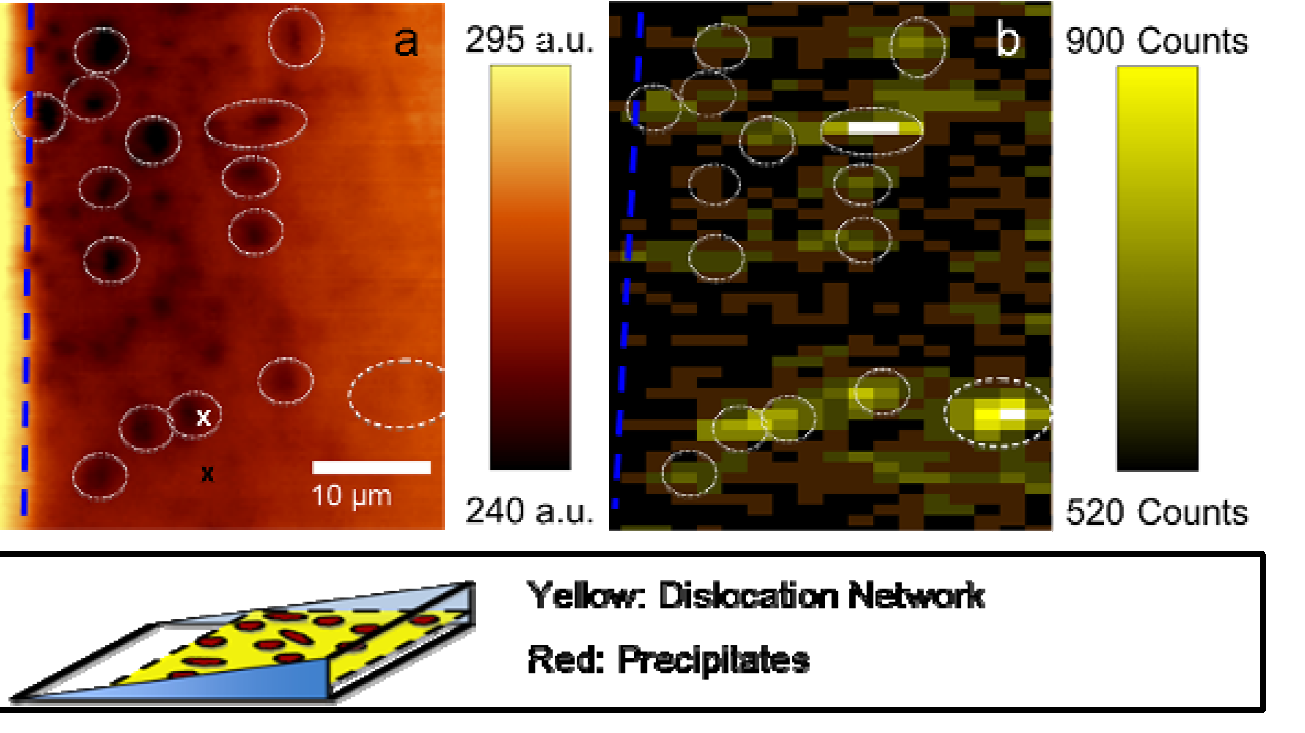
\includegraphics[width=15cm]{gundel_iron_precipitates}%
\caption[Iron precipitates]{Bottom: Scheme of the sample preparation with the polished angle. Top: A Intensity of the BB PL peak at room temperature (a), and of the iron X-ray K\alpha fluorecence (b) from \cite{gundel09}. The dislocation network intersects the surface to the right of the dashed blue line. The white circles show recombination active precipitates.}%
\label{fig:gundel_iron_precipitates}%
\end{figure}

Electron hole droplets (EHD), free excitons (FE) and bound excitons (BE) localized on phosphorus atoms has been steadily observed in \cite{drozdov03} with photoluminescence on samples with low-dislocated regions. When increasing dislocation density the FE, BE and EHD bands decrease sharply. This may be due exciton capture by dislocation lines D1,D2 and non-radiative recombination \cite{drozdov03}. EHD photoluminescence intensity is highly dependent on the pumping power \cite{satoshi04}. There is a linear dependence, and pumping with 3mW or less makes it hardly visible in \cite{satoshi04}.

Room temperature mapping of the 0.77eV band is attributed to oxygen precipitates in in thermally treated silicon made by the Czochralski process (Cz-Si) \cite{tajima95}. This band peak shifts parallel to the bandgap with temperature. The increase of this band on the dislocation lines is due to the preferential precipitation of oxygen \cite{tajima95}.

\cite{inoue07} state that the deep-level emission from multicrystalline silicon with an intensity maximum at 0.78eV at room temperature is diffrent from that of the D1 line at low temperature. Furthermore, \cite{inoue07} suggest that the 0.78eV emission is associated with oxygen precipitation, and that the intra-grain defects are dislocation clusters decorated with oxygen impurities in addition to heavy-metal impurities. \cite{gundel08} state that the origin of trap densities in multicrystalline silicon could be structural crystal defects, which are highly decorated with oxygen precipitates.

